\subsection{Referencia}

\subsubsection{Transmisión}

Se implementó en C++ y C\# la funcionalidad para transmitir los datos entre la Raspberry Pi y el software SettDev, que se ejecuta en el sistema operativo Windows; para este trabajo, se ejecutó en la versión Windows 10. Para la comunicación, se utilizó una trama TCP, cuya carga útil se muestra en la Figura \ref{fig:tramatcp}. Se utilizan dos bytes para el ángulo de la base, y un byte para cada ángulo de los eslabones, siendo 4 bytes en total.

\begin{figure}[htb]
	\centering
	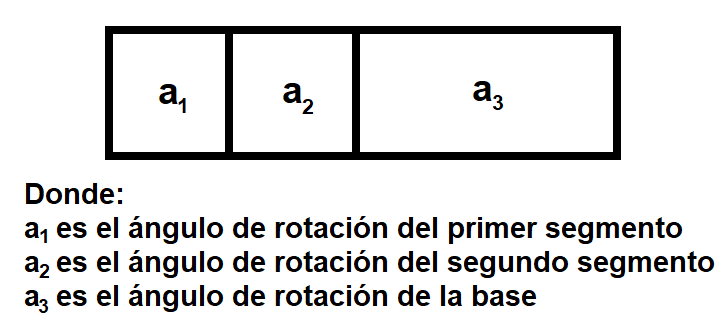
\includegraphics[scale=0.9]{tramatcp.png}
	\caption{Campo de datos de la trama TCP entre la Raspberry Pi y SettDev}
	\label{fig:tramatcp}
\end{figure}

\subsubsection{Simulación}

En la Figura \ref{fig:settdev} se observa la interfaz de usuario de SettDev. Éste se compone por módulos; cada módulo es un componente que interactúa con una característica en particular del PLC que se controla desde el software. La interfaz que se muestra, es el módulo desarrollado por personal de SEDPC para el proyecto; éste contiene un modelo en 3D de un brazo robótico, en el que las inclinaciones de cada una de sus articulaciones son modificadas por los controles deslizantes que aparecen en la parte superior del modelo.

\begin{figure}[htb]
	\centering
	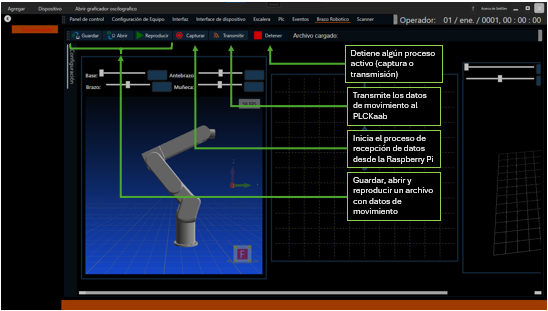
\includegraphics[scale=0.9]{settdev.png}
	\caption{Módulo de Brazo Robótico desarrollado por SEDPC}
	\label{fig:settdev}
\end{figure}

La Figura \ref{fig:referencia} muestra en detalle el brazo en 3D, modelado por personal de SEDPC. Este modelo tiene 2 grados de libertad (además del de la base), y un grado de libertad adicional para el efector final (Muñeca). Este brazo robótico recibirá los ángulos de inclinación de la etapa de Procesamiento y los reproducirá.

\begin{figure}[htb]
	\centering
	\includegraphics[scale=0.6]{referencia.png}
	\caption{Modelo de brazo en 3D utilizado como referencia}
	\label{fig:referencia}
\end{figure}